\documentclass[12pt, a4paper]{article}
\usepackage[utf8]{inputenc} %codification of the document

\usepackage{authblk}% This one is for adding affiliation of an author \affil command

%--------------------------
%Package for comment
\usepackage{comment}
%-------------------------------
%Package for coloring text
\usepackage{xcolor}

%---------------------------------

% Package for math

\usepackage{amsmath}
%------------------------------------------

% Package for images

\usepackage{graphicx}


%------------------------------------------

% Package for coding

\usepackage{listings}


%------------------------------------------
% Package for algorithms

\usepackage[ruled,vlined]{algorithm2e}


%------------------------------------------

%%For coloring and linking the reference and url. 
\usepackage{hyperref}
\hypersetup{
    colorlinks=true,
    linkcolor=blue,
    filecolor=magenta,      
    urlcolor=blue,
    pdftitle={Sharelatex Example},
    bookmarks=true,
    pdfpagemode=FullScreen,
}
%%---------------------------------
%% A macro is a shorthand for a more complicated sequence of commands. Later in the text, the macro can be used instead of those sequence of commands. 

\newcommand {\pr}{\textit{Projection,}$\pi$}
\newcommand {\se}{\textit{Selection,} $\sigma$}
\newcommand {\cp}{\textit{Cartesian product,}$\times$}
\newcommand {\un} {\textit{Union,}$\cup$}
\newcommand {\di}{\textit{Set difference,}$-$}
\newcommand {\re}{\textit{Rename,}$\rho$}

%----------------------------

%\begin{center}
%A thesis submitted to the Technical Faculty of IT and Design at Aalborg University (AAU) and the Department of Service and Information System Engineering at Universitat Politècnica de Catalunya (UPC), in partial fulfillment of the requirements within the scope of the IT4BI-DC programme for the joint Ph.D. degree in Computer Science. The thesis is not submitted to any other organization at the same time.
%\end{center}


%-------------------------


%-------------------------------
\begin{document}

\begin{titlepage}

\begin{figure}
	\centering
	\begin{minipage}[b]{0.15\textwidth}
		
\includegraphics[width=1\textwidth]{images/cu}
		%\caption{Black Image}
	\end{minipage} \hfill
	\end{figure}
	
\noindent%
  \begin{tabular}{@{}p{\textwidth}@{}}
    \hline
    \hline
    \vspace{0.2cm}
    \begin{center}
    \Huge{\textbf{
      Chittagong University Campus Event Management System
    }}
    \end{center}
    \vspace{0.2cm}\\
    \hline
    \hline
  \end{tabular}
  \vspace{4 cm}

\begin{center}
    {\large
      Database Project Report %Insert document type (e.g., Project Report)
    }\\
    \vspace{0.2cm}
    {\Large
      Group-37 % Insert group number
      
    }
  \end{center}
  \vfill
  
  \begin{center}
%  Report submitted December, 2021
  \end{center}
	\vfill
A project submitted to Dr. Rudra Pratap Deb Nath, Associate Professor, Department of Computer Science and Engineering, Chittagong University (CU) in partial fulfillment of the requirements for the Database Systems Lab course. The project is not submitted to any other organization at the same time. 

\end{titlepage}
\clearpage
%%%%% Details of student
%-------------------------
%Fill up the table with your group information
%----------------------------

\begin{table}[t]
\caption{Details of Group-01}% insert your group number 
\resizebox{\textwidth}{!}{%
\begin{tabular}{|l|l|l|l|l|}
\hline
Roll Id & Name & Sigature & Date & Supervisor Approval \\ \hline
        &      &          &      &                     \\ \hline
        &      &          &      &                     \\ \hline
        &      &          &      &                     \\ \hline
        &      &          &      &                     \\ \hline
        &      &          &      &                     \\ \hline
        &      &          &      &                     \\ \hline
\end{tabular}%
}
\end{table}
\clearpage






%-------------------------

% Showing contents as an Index
\setcounter{secnumdepth}{5}
\setcounter{tocdepth}{5}
\tableofcontents
\listoffigures

\listoftables
\lstlistoflistings
%-----------------------



%
%\begin{abstract}
The summary of your project
Explain the following each point with at most two sentences: \texttt{Motivation:} Why are you doing this database project? Why does it motivate you? \texttt{Define the problem:} What is the problem you choose?  \texttt{Limitations of current solutions:} What are current problems faced by the stack-holders? Your approach to fill the gap: What are the processes you will use to develop your solution? \texttt{Your solution: }What solution will your system provide? Evaluation of your solution: How will you evaluate your solution? \texttt{The significance of your project, limitation and future work in short}
\end{abstract}
\clearpage
%% Maintain the consistency.
% Maintain a good writing flow. 

\section{Introduction}\label{sec:introduction}
Explain from abstract level:
Write why you are doing this project and writing this document. 

The objective of this course is to develop a database application system by applying the theories, methodologies, tools, and technologies we learnt in [write database course theory code and name].  


\subsection{Background and Motivation}\label{subsec:bm}
Write the background and motivation of project. What is the current state of the problem? What are the problems currently faced by the stack holders? What is your approach to solve/address the problems? Write the significance of your solution.   

\subsection{Problem Statement}\label{subsec:ps} Precisely state your problem statement, i.e., what is the problem and what you are going to address. Technically mention the entity types or relationships in the statement

\subsection{System Definition}\label{subsec:sd} 
Also write a system definition: A concise description of a computerized system ( that you are about to develop) expressed in natural language

A system definition example of a Conference planning system

\textit{``A computerized system used to control the ICCIT conference by registering participants and their payments to organizers using invoicing and other reporting methods. Controlling should be easy to learn, as ICCIT conferences use unpaid and untrained labor."}


\subsection{System Development Process}\label{subsec:sdp}
Write the system development process. Try to use a figure to describe the process. In brief, the  steps are 1) Requirement gathering and analysis, 2) Database modeling: conceptual modeling, logical modeling, and normalization, 3) System architecture, 4) Implementation, and 5) Validation. Briefly describe each step. Remember the output of a step is the  input of the immediate next step. Write that each step of the system development process will be a separate section of this document.
\begin{comment}


To design a database, one should follow the following steps:
\begin{enumerate}
\item Requirement analysis
	\begin{itemize}
		\item[-] interviewing, documentation, etc .
	\end{itemize}

\item Mapping onto a conceptual model (conceptual design)
     \begin{itemize}
     	\item[-] ER model
     \end{itemize}
\item Mapping onto a data model (logical design)
	\begin{itemize}
     	\item[-] Relational model, object model etc. 
     \end{itemize}
\item Normalization
\item System Architecture
\item Realization and Implementation (physical design)    
    
\end{enumerate}
\end{comment}


\subsection{Organization} Write the organization of the document here. For example: Section~\ref{sec:introduction} gives the overview of the project, Section~\ref{sec:projectmanagement} describes how the project and the resources are managed. .........Finally, the conclusion and the pointers to the future work are outlined in Section~~\ref{sec:cfw}.

\clearpage
%\section{Project Management}\label{sec:projectmanagement}
Describe how the projects are resources are organized and managed in details, the roles of each members, used tools (Github, Trello ect.). See the scrum method. 
\clearpage
\section{Requirement Gathering and Analysis}

Requirement analysis in this project involves identifying the data that needs to be stored in the database and understanding how it will be accessed by different users. The system is being developed after discussing needs with one of the campus event organizers. Ensuring clear and complete requirements before beginning is essential for creating a system that meets the needs of all stakeholders.

\subsection{Process of Requirement Analysis}

\subsubsection{Discussion with an Event Organizer and students}

Discussions with an event organizer and a student form the core of the analysis. Through these conversations, the aim is to identify the problems encountered in organizing campus events, managing attendees, and allocating resources. Below are some key points from the discussion.
\begin{itemize}
    \item \textbf{Question 1:} What are some challenges in managing events and facilitating connections among students and teachers?

        \item \textbf{Event Organizer:} We face issues organizing events across various interests, as we have to coordinate with departments and manage resources like locations and materials. Also, students may not know about events that match their interests, limiting opportunities to connect.
 
    
    \item \textbf{Question 2:} How does the current system limit participant engagement?

        \item \textbf{Student:} Without a centralized platform, it’s challenging to keep track of events and connect with others who share similar interests. We want a way to see all available events, know who’s attending, and connect with participants after events.

    
    \item \textbf{Question 3:} What improvements would you like to see in event notifications and updates?

        \item \textbf{Event Organizer:} Notifications for event updates, changes, or cancellations should be instant and accessible. Participants often don’t get updates in time, which can make engagement difficult.

\end{itemize}

\subsubsection{Understanding the Requirement}

After discussing these points, it was concluded that the system must handle all event-related data automatically, minimizing errors and delays. The system should allow organizers and participants to manage and access information seamlessly and ensure reliable, timely communication of updates.

Basic information requirements identified are:
\begin{itemize}
    \item \textbf{Event Information}: Event name, date, time, location, and organizer.
    \item \textbf{Participant Information}: Name, ID, email.
    % \item \textbf{Resource Information}: Type, availability, and quantity of resources.
    \item \textbf{Location Information}: area details, capacity, and availability for booking.
\end{itemize}

\subsection{Identifying Stakeholders}

Since the system is being developed to address event management challenges faced on campus, the key stakeholders are:

\begin{itemize}
    \item \textbf{Event Organizers} (teachers, students, and staff involved in planning and managing events).
    \item \textbf{Participants} (students, teachers).
    \item \textbf{Campus Administration} (managing location bookings and maintaining event records).
    % \item \textbf{IT Support Staff} (ensuring the smooth operation and maintenance of the system).
\end{itemize}

As the Question , I aim to create a solution that is user-friendly and effective for all stakeholders.

\subsection{System Specification}

After analyzing requirements and identifying stakeholders, a \textbf{web-based system} has been selected for development. The next step is to design a conceptual model, focusing on a high-level view to confirm that it aligns with the specified requirements.

The system will include features for event creation, participant registration, resource management, and real-time notifications, ensuring that all necessary information is accessible and manageable for everyone involved.



% \section{Requirement Gathering and Analysis}
% The campus event management system aims to connect students and teachers through campus events by facilitating the process of creating, joining, and managing events across a variety of interests, such as adventure, sports, and more. The system is inspired by platforms like Meetup.com, allowing users to discover events, connect with others, and join communities around shared interests. Requirements are developed after discussions with campus stakeholders to ensure it meets the needs of organizers and participants alike.

% \subsection{Process of Requirement Analysis}
% \subsubsection{Discussions with Event Organizers and Students}
% Conversations with campus event organizers and students help to identify challenges in event management and understand the requirements for a system that encourages active participation and connection.

% \begin{itemize}
%     \item \textbf{Question 1:} What are some challenges in managing events and facilitating connections among students and teachers?

%         \item \textbf{Event Organizer:} We face issues organizing events across various interests, as we have to coordinate with departments and manage resources like locations and materials. Also, students may not know about events that match their interests, limiting opportunities to connect.
 
    
%     \item \textbf{Question 2:} How does the current system limit participant engagement?

%         \item \textbf{Student:} Without a centralized platform, it’s challenging to keep track of events and connect with others who share similar interests. We want a way to see all available events, know who’s attending, and connect with participants after events.

    
%     \item \textbf{Question 3:} What improvements would you like to see in event notifications and updates?

%         \item \textbf{Event Organizer:} Notifications for event updates, changes, or cancellations should be instant and accessible. Participants often don’t get updates in time, which can make engagement difficult.

% \end{itemize}

% \subsubsection{Understanding the Requirements}
% Based on these discussions, the campus event management system should simplify the event creation and joining process and foster communication among users. Key requirements include:

% \begin{itemize}
%     \item \textbf{Event Discovery and Connection:} Enable students and teachers to easily find events that match their interests and see who else is attending.
%     \item \textbf{Participant Engagement:} Allow participants to connect before, during, and after events, encouraging a community of shared interests.
%     \item \textbf{Timely Notifications:} Ensure that participants receive timely updates about any event changes or new opportunities.
% \end{itemize}

% \subsection{Identifying Stakeholders}
% The system is designed to connect users and enhance event participation on campus. Key stakeholders include:

% \begin{itemize}
%     \item \textbf{Event Organizers} (teachers, students, and staff organizing campus activities).
%     \item \textbf{Participants} (students, faculty, and guests attending events).
%     \item \textbf{Campus Administration} (overseeing event logistics and venue availability).
% \end{itemize}

% The goal is to create a platform that is intuitive and effective for all users, encouraging students and faculty to engage with one another through campus events.

% \subsection{System Specification}
% Following the analysis, a web-based platform was chosen to best support the event management needs. The system will include features for event creation, participant registration, and real-time notifications to make all event-related information accessible to users, enhancing their ability to connect through shared interests.

% %\section{Conceptual Modelling}\label{sec:cm}
% %Conceptually model your database using an E-R diagram. Use the legends in your diagram. Write how you find the entity types, relationships, and attributes from Section~\ref{sec:rga}


% \section{Conceptual Modeling}

% The next step after requirement analysis is conceptual modeling. Conceptual modeling is the process of developing an abstract model or graphical representation using real-world concepts or ideas. It is a high-level diagram that defines, describes, organizes, and presents data elements and their relationships with relatively few details. 

% For this project, the Entity Relationship Model (ERM) was chosen as it is widely used and was emphasized in our course. ERM provides a clear and organized way to represent data structures, which is essential for the campus event management system.

% \subsection{Entity-Relationship Model}

% An Entity-Relationship Diagram (ERD) shows the relationships of entities stored in a database. ER diagrams explain the logical structure of a database and illustrate how entities interact. In ER diagrams, three basic concepts are used:

% \begin{enumerate}
%     \item \textbf{Entity}: In database management systems, an entity is a data object that represents a real-world object or concept, such as an event or a participant. Entities are often represented as tables, with each row representing a specific instance. Entities are shown in rectangular shapes in the ER model.

%     \item \textbf{Attribute}: An attribute represents a characteristic or property of an entity. For example, attributes for an event entity might include \textit{event name}, \textit{date}, and \textit{location}. Attributes are represented by oval shapes in the ER model.

%     \item \textbf{Relationship}: Relationships are connections between entities that define how data in one entity relates to data in another. In the ER diagram, relationships between entities are represented by diamonds and are labeled to describe the interaction. Common types of relationships include:
%     \begin{enumerate}
%         \item One-to-One
%         \item One-to-Many
%         \item Many-to-One
%         \item Many-to-Many
%     \end{enumerate}
% \end{enumerate}

% \subsection{Detailing the Entity-Relationship Model}

% From the analysis, the following entities and relationships have been identified for the Campus Event Management System:

% \subsubsection{Entity Types}

% \begin{enumerate}
%     \item \textbf{User}: Represents users of the system with attributes such as \textit{user\_id}, \textit{username}, \textit{email}, \textit{password}, \textit{user\_type}, \textit{created\_at}, \textit{last\_login},and \textit{contact\_number}.
%     \item \textbf{Event}: Represents each campus event, including attributes like \textit{event\_id}, \textit{event\_name}, \textit{description}, \textit{event\_date}, \textit{start\_time}, \textit{end\_time}, \textit{location\_id}, \textit{organizer\_id}, \textit{status}, and \textit{max\_attendees}.
    
%     % adding teacher and student
%     \item \textbf{Teacher}: Represents faculty members involved in events, including attributes like \textit{teacher\_id}, \textit{name}, \textit{email}, \textit{department}, \textit{phone\_number}, and \textit{user\_id}.
    
%     \item \textbf{Student}: Represents students who may attend events, including attributes like \textit{student\_id}, \textit{name}, \textit{email}, \textit{enrollment\_year}, \textit{major}, and \textit{user\_id}.
    
%     \item \textbf{Organizer}: Represents individuals organizing events with attributes such as \textit{organizer\_id}, \textit{name}, \textit{contact\_number}, \textit{email}, \textit{user\_id}, and \textit{organization}.
%     % \item \textbf{Participant}: Represents people attending events, including attributes like \textit{participant\_id}, \textit{event\_id}, \textit{user\_id}, \textit{registration\_date}, and \textit{status}.
%     \item \textbf{Location}: Represents locations where events are held, with attributes like \textit{location\_id}, \textit{room\_name}, \textit{building}, \textit{capacity}, and \textit{availability\_status}.
%     % \item \textbf{Resource}: Represents resources allocated for events, including attributes like \textit{resource\_id}, \textit{resource\_type}, \textit{quantity}, \textit{availability\_status}, and \textit{location\_id}.
%     % \item \textbf{Booking}: Represents the booking of locations and resources, with attributes like \textit{booking\_id}, \textit{event\_id}, \textit{location\_id}, \textit{resource\_id}, \textit{start\_time}, and \textit{end\_time}.
%     % \item \textbf{Notification}: Represents notifications sent to users with attributes like \textit{notification\_id}, \textit{user\_id}, \textit{event\_id}, \textit{message}, \textit{notification\_date}, and \textit{status}.
% \end{enumerate}

% \subsubsection{Relationship Types}

% The relationships between the entities identified in the ER model are as follows:

% \begin{itemize}
%     \item \textbf{Organized by}: Connects \textit{Organizer} and \textit{Event} entities, where each organizer can manage multiple events.
%     \item \textbf{Registers}: Connects \textit{Participant} and \textit{Event} entities, where a participant can register for multiple events, and each event can have multiple participants.
%     % \item \textbf{Requires}: Connects \textit{Event} and \textit{Resource} entities, where an event may require multiple resources, and each resource can be allocated to multiple events.
%     \item \textbf{Located At}: Connects \textit{Event} and \textit{Location} entities, where each event is held in a specified location.
% \end{itemize}
% \begin{figure}[h]
%     \centering
%     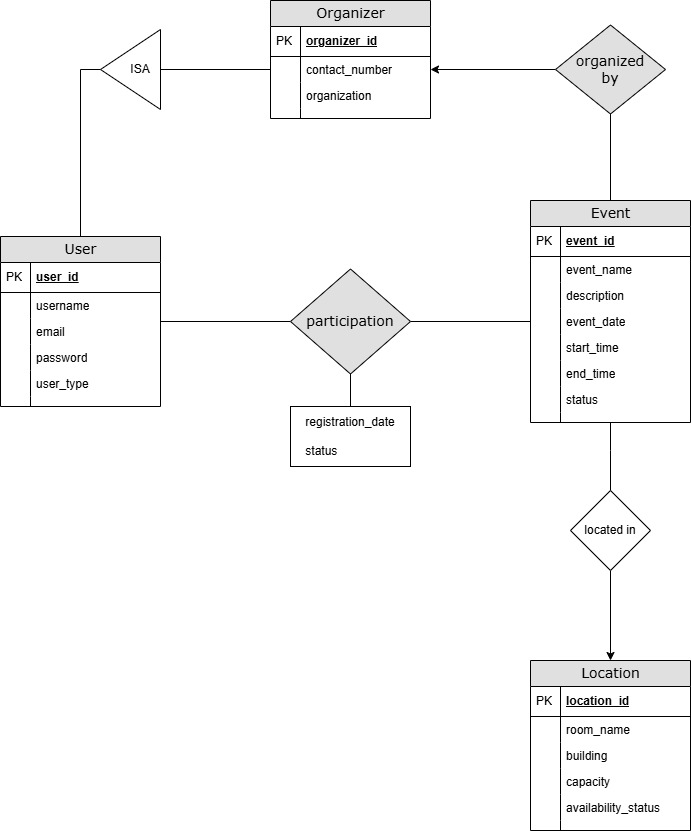
\includegraphics[scale=0.4]{images/Event_Management2.jpg}
% \end{figure}
% In the figure the ER diagram displays these entity types and their relationships. For instance, the relationship between \textbf{Event} and \textbf{Participant} indicates that one participant can register for multiple events. The \textbf{Organizer} manages one or more events, and resources are allocated to events as needed.

% Entities are represented in rectangular shapes, relationships in diamond shapes, and attributes in oval shapes.


\section{Conceptual Model for Campus Event Management System}

The conceptual model for the Campus Event Management System was developed using the Entity-Relationship Model (ERM). The ERM was chosen because of its clarity in representing data structures and its relevance to our coursework. ER diagrams define the logical structure of the database, showing how data elements and their relationships interact within the system.

\subsection{Entity-Relationship Model}

An \textbf{Entity-Relationship Diagram (ERD)} visually represents the data structure of the Campus Event Management System, showing how entities and their attributes relate to each other.

\textbf{Key Concepts in the ER Model:}

\begin{itemize}
    \item \textbf{Entity}: An entity represents a real-world object or concept, like an event or user. Entities are represented as tables in the database, with each row representing a specific instance.
    \item \textbf{Attribute}: Attributes represent the properties or characteristics of an entity. For example, attributes of the \texttt{Event} entity include \texttt{event\_name}, \texttt{event\_date}, and \texttt{location\_id}.
    \item \textbf{Relationship}: Relationships define the interactions between entities. Common types of relationships include:
    \begin{itemize}
        \item \textbf{One-to-One}
        \item \textbf{One-to-Many}
        \item \textbf{Many-to-One}
        \item \textbf{Many-to-Many}
    \end{itemize}
\end{itemize}

\subsection{Detailing the Entity-Relationship Model}

From the analysis, the following \textbf{entities} and \textbf{relationships} have been identified for the Campus Event Management System.

\subsubsection{Entity Types}

\begin{enumerate}
    \item \textbf{User}: Represents users of the system with attributes:
    \begin{itemize}
        \item \texttt{username} (Primary Key)
        \item \texttt{name}
        \item \texttt{email}
        \item \texttt{password}
        \item \texttt{user\_type} (enum: `student`, `teacher`)
        \item \texttt{contact\_number}
    \end{itemize}

    \item \textbf{Student}: Represents students who may attend events, with attributes:
    \begin{itemize}
        \item \texttt{student\_id} (Primary Key)
        \item \texttt{enrollment\_date}
        \item \texttt{username} (Foreign Key referencing \texttt{User.username})
        \item \texttt{department}
    \end{itemize}

    \item \textbf{Teacher}: Represents faculty members involved in events, with attributes:
    \begin{itemize}
        \item \texttt{teacher\_id} (Primary Key)
        \item \texttt{employment\_date}
        \item \texttt{username} (Foreign Key referencing \texttt{User.username})
    \end{itemize}

    \item \textbf{Event}: Represents each campus event, with attributes:
    \begin{itemize}
        \item \texttt{event\_id} (Primary Key)
        \item \texttt{event\_name}
        \item \texttt{description}
        \item \texttt{event\_date}
        \item \texttt{start\_time}
        \item \texttt{end\_time}
        \item \texttt{status} (enum: `pending`, `ongoing`, `finished`)
        \item \texttt{max\_attendees}
        \item \texttt{currently\_registered}
        \item \texttt{category\_id} (Foreign Key referencing \texttt{Event\_Category.category\_id})
        \item \texttt{location\_id} (Foreign Key referencing \texttt{Location.location\_id})
    \end{itemize}

    \item \textbf{Location}: Represents locations where events are held, with attributes:
    \begin{itemize}
        \item \texttt{location\_id} (Primary Key)
        \item \texttt{address}
        \item \texttt{description}
        \item \texttt{is\_available}
    \end{itemize}

    \item \textbf{Event Category}: Represents categories for events, with attributes:
    \begin{itemize}
        \item \texttt{category\_id} (Primary Key)
        \item \texttt{category\_name}
    \end{itemize}
\end{enumerate}

\subsubsection{Relationship Types}

The relationships between the entities are as follows:

\begin{itemize}
    \item \textbf{Organized\_By}: Connects \texttt{User} and \texttt{Event}, where each user (acting as an organizer) can manage multiple events.
    \begin{itemize}
        \item \texttt{username} (Foreign Key referencing \texttt{User.username})
        \item \texttt{event\_id} (Foreign Key referencing \texttt{Event.event\_id})
    \end{itemize}

    \item \textbf{Registers}: Connects \texttt{User} (as a participant) and \texttt{Event}, where a participant can register for multiple events, and each event can have multiple participants.
    \begin{itemize}
        \item \texttt{username} (Foreign Key referencing \texttt{User.username})
        \item \texttt{event\_id} (Foreign Key referencing \texttt{Event.event\_id})
        \item \texttt{registration\_date}
    \end{itemize}

    \item \textbf{Located At}: Connects \texttt{Event} and \texttt{Location}, where each event is held at a specified location.
    \begin{itemize}
        \item \texttt{location\_id} (Foreign Key referencing \texttt{Location.location\_id})
        \item \texttt{event\_id} (Foreign Key referencing \texttt{Event.event\_id})
    \end{itemize}
\end{itemize}
\newpage
\begin{figure}[h]
    \centering
    \hspace*{-2.5cm} % Adjust this value for the desired left margin
    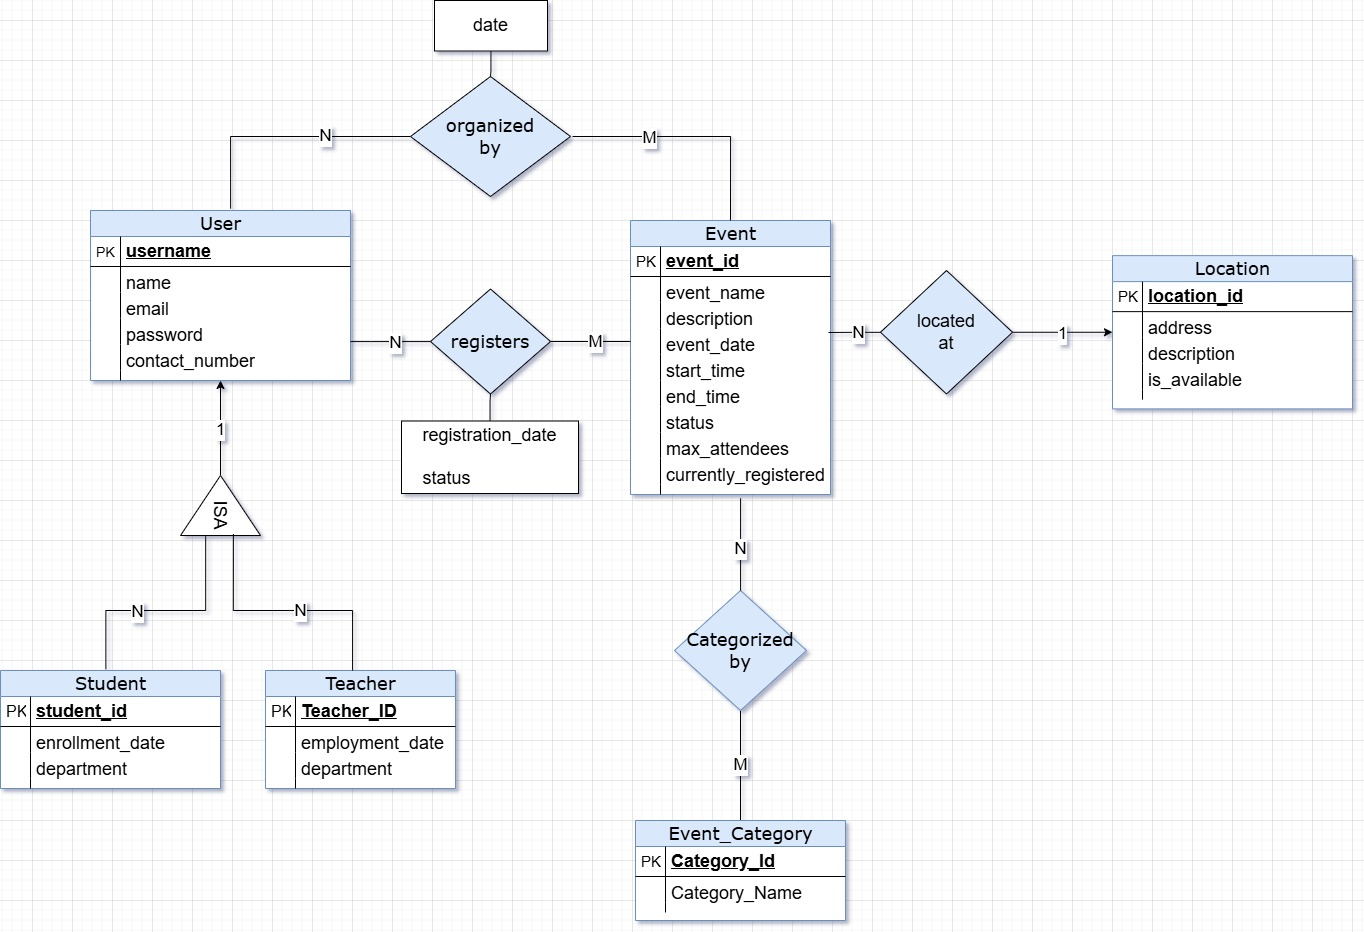
\includegraphics[scale=.4]{images/er_diagram.jpg}
\end{figure}


This ER model provides a high-level structure for managing campus events, representing how data is organized within the Campus Event Management System. The relationships between entities allow efficient linking of users, events, locations, and categories, facilitating seamless interactions within the system.
\clearpage
%\section{Logical Modelling}\label{sec:lm}
After defining the conceptual model, we proceed with the logical data model for the Campus Event Management System.
The logical model outlines the structure of the data items and their relationships in a formal way.
For our system, we use the relational model.
\subsection{Relational Model}
In a relational model, data and their relationships are represented through a collection of interlinked tables.
Each table contains rows and columns, where each column represents an attribute of an entity, and each row holds a record.
The relational schema defines how each table (relation) is structured, specifying the table name and a list of attribute names, each tied to a specific domain.

\subsubsection{Tables and Attributes}

\begin{itemize}
    \item \textbf{User} \\
        \texttt{user(username, username, email, password, user\_type,contact\_number)} \\
        \textbf{Primary Key:} username \\

    \item \textbf{Student} \\
        \texttt{student(student\_id, enrollment\_date, username)} \\
        \textbf{Primary Key:} student\_id \\
        \textbf{Foreign Key:} username $\rightarrow$ user(username)
    
    \item \textbf{Teacher} \\
        \texttt{teacher(teacher\_id, employment\_date, username)} \\
        \textbf{Primary Key:} teacher\_id \\
        \textbf{Foreign Keys:} \\
        \hspace*{1cm} username $\rightarrow$ user(username)
    
    \item \textbf{Venue} \\
        \texttt{Venue(venue\_id, venue\_name)} \\
        \textbf{Primary Key:} venue\_id
    

    \item \textbf{Location} \\
        \texttt{location(location\_id, location\_name)} \\
        \textbf{Primary Key:} location\_id
        
    \item \textbf{Event\_Category} \\
        \texttt{event\_category(category\_id, category\_name)} \\
        \textbf{Primary Key:} category\_id
        
    \item \textbf{Event} \\
        \texttt{event(event\_id, event\_name, description, event\_date, start\_time, end\_time, status, max\_attendees, category\_id, venue\_id)} \\
        \textbf{Primary Key:} event\_id \\
        \textbf{Foreign Keys:} \\
        \hspace*{1cm} category\_id $\rightarrow$ event\_category(category\_id) \\
        \hspace*{1cm} venue\_id $\rightarrow$ Venue(venue\_id)
        
    \item \textbf{Registers} \\
        \texttt{registers(username, event\_id, registration\_date)} \\
        \textbf{Primary Key:} (username, event\_id) \\
        \textbf{Foreign Keys:} \\
        \hspace*{1cm} username $\rightarrow$ user(username) \\
        \hspace*{1cm} event\_id $\rightarrow$ event(event\_id)
        
    \item \textbf{Organized\_By} \\
        \texttt{organized\_by(username, event\_id)} \\
        \textbf{Primary Key:} (username, event\_id) \\
        \textbf{Foreign Keys:} \\
        \hspace*{1cm} username $\rightarrow$ user(username) \\
        \hspace*{1cm} event\_id $\rightarrow$ event(event\_id)
\end{itemize}

\clearpage


% \section{Logical Modeling}

% After defining the conceptual model, we proceed with the logical data model for the Campus Event Management System.
% The logical model outlines the structure of the data items and their relationships in a formal way.
% For our system, we use the relational model.

% \subsection{Relational Model}

% In a relational model, data and their relationships are represented through a collection of interlinked tables.
% Each table contains rows and columns, where each column represents an attribute of an entity, and each row holds a record.
% The relational schema defines how each table (relation) is structured, specifying the table name and a list of attribute names, each tied to a specific domain.

% \subsection{ER Model to Relational Schema}

% The following steps were used to map our ER model to the relational schema:

% \begin{enumerate}
%     \item Each entity type is converted to a table, with each entity attribute becoming a column.
%     \item A primary key is assigned to each table to uniquely identify each row. The primary key may be a single attribute or a combination of attributes.
%     \item For a many-to-many relationship, a separate relationship table is created. This table has a composite primary key, consisting of the primary keys of the linked entities, and any additional attributes specific to the relationship.
%     \item In a one-to-one relationship, the primary key of either entity is added as a foreign key to the other. For one-to-many or many-to-one relationships, the foreign key from one side is added to the many side.
% \end{enumerate}

% In our database schema for the \texttt{campus\_event} system, all user-related information (such as student or teacher details) is stored in the \texttt{user} table, where \texttt{username} is the primary key. This table includes attributes like \texttt{username}, \texttt{name}, \texttt{email}, \texttt{password}, \texttt{user\_type}, and \texttt{contact\_number}.

% The \texttt{event} table holds details of each campus event, including attributes such as \texttt{event\_id} (primary key), \texttt{event\_name}, \texttt{description}, \texttt{event\_date}, \texttt{start\_time}, \texttt{end\_time}, \texttt{status}, \texttt{max\_attendees},\\
% \texttt{currently\_registered}, \texttt{category\_id}, and \texttt{location\_id}. \texttt{category\_id} and \texttt{location\_id} are foreign keys referencing the \texttt{event\_category} and \texttt{location} tables, respectively.

% Since there is a many-to-many relationship between \texttt{user} and \texttt{event} (as multiple users can register for multiple events), we have a \texttt{registers} table. This table uses a composite primary key made up of \texttt{username} and \texttt{event\_id} to uniquely identify each registration. Additionally, it includes the attribute \texttt{registration\_date} to store the date of each registration.

% The \texttt{organized\_by} table represents the relationship between organizers (users) and events they manage, with \texttt{username} and \texttt{event\_id} as a composite primary key. In this table, \texttt{username} references the primary key in the \texttt{user} table, while \texttt{event\_id} references the primary key in the \texttt{event} table.

% There is also a one-to-many relationship between \texttt{event} and \texttt{user}, where each \texttt{event} can be created by a user with a specific \texttt{username}.

% \subsection{List of Relational Schemas for Our System}

% \begin{itemize}
%     \item \texttt{user(username, name, email, password, user\_type, contact\_number)}
%     \item \texttt{student(student\_id, enrollment\_date, username, department)}
%     \item \texttt{teacher(teacher\_id, employment\_date, username)}
%     \item \texttt{event(event\_id, event\_name, description, event\_date, start\_time, end\_time, status, max\_attendees, currently\_registered, category\_id, location\_id)}
%     \item \texttt{event\_category(category\_id, category\_name)}
%     \item \texttt{location(location\_id, address, description, is\_available)}
%     \item \texttt{registers(username, event\_id, registration\_date)}
%     \item \texttt{organized\_by(username, event\_id)}
% \end{itemize}

% This relational schema provides a structured view of the Campus Event Management System, detailing each table’s attributes and their relationships in the database.

%% \section{Normalization}\label{sec:norm}

% \section*{Database Schema}
% The following database schema is used in the campus event management system:

% \begin{itemize}
%     \item \textbf{department(department\_id, department\_name)}
%     \item \textbf{user(user\_id, username, email, password, user\_type, department\_id, contact\_number)}
%     \item \textbf{student(student\_id, enrollment\_date, user\_id)}
%     \item \textbf{teacher(teacher\_id, employment\_date, department\_id, user\_id)}
%     \item \textbf{location(location\_id, room\_number, building, capacity, is\_available)}
%     \item \textbf{event\_category(category\_id, category\_name)}
%     \item \textbf{event(event\_id, event\_name, description, event\_date, start\_time, end\_time, status, max\_attendees, currently\_registered, category\_id, location\_id)}
%     \item \textbf{registers(user\_id, event\_id, registration\_date)}
%     \item \textbf{organized\_by(user\_id, event\_id)}
% \end{itemize}

% \section*{Normalization Proof}

% \subsection*{First Normal Form (1NF)}
% To satisfy 1NF:
% \begin{itemize}
%     \item Each column must contain atomic (indivisible) values.
%     \item Each table must have a unique primary key.
% \end{itemize}

% \noindent \textbf{Proof:} Each table in the schema has atomic columns, with no repeating groups or arrays, and each row is uniquely identified by a primary key in each table. Therefore, the schema is in 1NF.

% \subsection*{Second Normal Form (2NF)}
% To satisfy 2NF:
% \begin{itemize}
%     \item The schema must be in 1NF.
%     \item All non-key attributes must depend on the whole primary key (no partial dependencies).
% \end{itemize}

% \noindent \textbf{Proof:} All tables with a single primary key automatically satisfy 2NF since there are no partial dependencies. Tables with composite primary keys (\textbf{registers} and \textbf{organized\_by}) also satisfy 2NF, as each non-key attribute depends on the entire composite primary key. Therefore, the schema is in 2NF.

% \subsection*{Third Normal Form (3NF)}
% To satisfy 3NF:
% \begin{itemize}
%     \item The schema must be in 2NF.
%     \item There should be no transitive dependencies, meaning non-key attributes must depend only on the primary key.
% \end{itemize}

% \noindent \textbf{Proof:} Each non-key attribute in each table depends only on the primary key:
% \begin{itemize}
%     \item In the \textbf{user} table, \texttt{department\_id} references the \textbf{department} table without any transitive dependencies, as departments are stored in a separate table.
%     \item In the \textbf{event} table, \texttt{category\_id} and \texttt{location\_id} reference separate tables (\textbf{event\_category} and \textbf{location}), avoiding any transitive dependencies.
% \end{itemize}
% Since each table in the schema is in 2NF and has no transitive dependencies, the schema is in 3NF.

% \subsection*{Boyce-Codd Normal Form (BCNF)}
% To satisfy BCNF:
% \begin{itemize}
%     \item The schema must be in 3NF.
%     \item Every determinant must be a candidate key.
% \end{itemize}

% \noindent \textbf{Proof:} In each table, there are no partial or transitive dependencies, and all non-key attributes depend solely on candidate keys. As such, the schema adheres to BCNF.

% \section*{Conclusion}
% The schema is normalized up to Boyce-Codd Normal Form (BCNF). Each table in the schema adheres to the requirements of 1NF, 2NF, 3NF, and BCNF, ensuring data integrity and eliminating redundancy.

% \clearpage



% \subsection{Normalization Analysis}

% \subsubsection{user Table}
% \begin{itemize}
%     \item \textbf{Primary Key:} username
%     \item \textbf{Functional Dependencies:} \texttt{username} $\rightarrow$ \texttt{name, email, password, user\_type, department, contact\_number}
%     \item \textbf{Normalization:}
%     \begin{itemize}
%         \item \textbf{3NF:} Each non-key attribute depends only on \texttt{username}, so it's in 3NF.
%         \item \textbf{BCNF:} Since \texttt{username} is the only candidate key, it is also in BCNF.
%     \end{itemize}
% \end{itemize}

% \subsubsection{student Table}
% \begin{itemize}
%     \item \textbf{Primary Key:} student\_id
%     \item \textbf{Functional Dependencies:} \texttt{student\_id} $\rightarrow$ \texttt{enrollment\_date, username}
%     \item \textbf{Normalization:}
%     \begin{itemize}
%         \item \textbf{3NF:} Each non-key attribute depends only on \texttt{student\_id}, so it's in 3NF.
%         \item \textbf{BCNF:} As \texttt{student\_id} is the only candidate key, it is also in BCNF.
%     \end{itemize}
% \end{itemize}

% \subsubsection{teacher Table}
% \begin{itemize}
%     \item \textbf{Primary Key:} teacher\_id
%     \item \textbf{Functional Dependencies:} \texttt{teacher\_id} $\rightarrow$ \texttt{employment\_date, username}
%     \item \textbf{Normalization:}
%     \begin{itemize}
%         \item \textbf{3NF:} Each non-key attribute depends only on \texttt{teacher\_id}, so it's in 3NF.
%         \item \textbf{BCNF:} With \texttt{teacher\_id} as the only candidate key, it is also in BCNF.
%     \end{itemize}
% \end{itemize}

% \subsubsection{location Table}
% \begin{itemize}
%     \item \textbf{Primary Key:} location\_id
%     \item \textbf{Functional Dependencies:} \texttt{location\_id} $\rightarrow$ \texttt{address, description, is\_available}
%     \item \textbf{Normalization:}
%     \begin{itemize}
%         \item \textbf{3NF:} Each non-key attribute depends only on \texttt{location\_id}, so it’s in 3NF.
%         \item \textbf{BCNF:} With \texttt{location\_id} as the only candidate key, it is also in BCNF.
%     \end{itemize}
% \end{itemize}

% \subsubsection{event Table}
% \begin{itemize}
%     \item \textbf{Primary Key:} event\_id
%     \item \textbf{Functional Dependencies:} \texttt{event\_id} $\rightarrow$ \texttt{event\_name, description, event\_date, start\_time, end\_time, status, max\_attendees, currently\_registered, category\_id, location\_id}
%     \item \textbf{Normalization:}
%     \begin{itemize}
%         \item \textbf{3NF:} Each non-key attribute depends only on \texttt{event\_id}, so it’s in 3NF.
%         \item \textbf{BCNF:} Since \texttt{event\_id} is the only candidate key, it is also in BCNF.
%     \end{itemize}
% \end{itemize}

% \subsubsection{registers Table}
% \begin{itemize}
%     \item \textbf{Primary Key:} (username, event\_id)
%     \item \textbf{Functional Dependencies:} (username, event\_id) $\rightarrow$ \texttt{registration\_date}
%     \item \textbf{Normalization:}
%     \begin{itemize}
%         \item \textbf{3NF:} Each non-key attribute depends only on the composite key (username, event\_id), so it’s in 3NF.
%         \item \textbf{BCNF:} There are no additional candidate keys, so it’s in BCNF.
%     \end{itemize}
% \end{itemize}

% \subsubsection{organized\_by Table}
% \begin{itemize}
%     \item \textbf{Primary Key:} (username, event\_id)
%     \item \textbf{Functional Dependencies:} (username, event\_id) $\rightarrow$ \texttt{None}
%     \item \textbf{Normalization:}
%     \begin{itemize}
%         \item \textbf{3NF and BCNF:} It’s a junction table with no non-key attributes, so it’s automatically in BCNF.
%     \end{itemize}
% \end{itemize}





\section{Normalization of Database Tables}

Normalization is a process used to minimize or remove data redundancy in a set of relations. The primary goal of normalization is to eliminate anomalies that can occur during data insertion, update, or deletion, thus making the database consistent, dependency-preserving, and free of redundancy. Below, we analyze the normalization forms (specifically 3NF) for each table in the campus event management database.

\subsection{Normalizing user Table}

The \texttt{user} table has the attributes:
\[
\{ \texttt{username}, \texttt{name}, \texttt{email}, \texttt{password}, \texttt{user\_type}, \texttt{contact\_number} \}
\]
\begin{figure}[h]
    \centering
    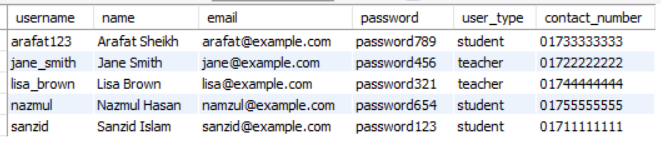
\includegraphics[scale=0.7]{images/table_data/user_table.png}
\end{figure}
% \csvautotabular{table_data/user.csv}

% \pgfplotstabletypeset[
%     col sep=comma, % Define column separator
%     header=true, % Use the first row as headers
%     every head row/.style={before row=\hline, after row=\hline}, % Add horizontal lines
%     every last row/.style={after row=\hline}
% ]{table_data/user.csv} 


Based on the demo data, we identify the following functional dependencies and analyze the candidate keys, 
prime attributes, and non-prime attributes to determine its normalization status.

\begin{itemize}
    \item \textbf{Functional Dependencies:}
    \begin{itemize}
        \item \texttt{\underline{username}} $\rightarrow$ \texttt{username,name, email, password, user\_type, contact\_number}
    \end{itemize}
    \begin{itemize}
        \item \texttt{email}$\rightarrow$ \texttt{username,name, email, password, user\_type, contact\_number}
    \end{itemize}
    \begin{itemize}
        \item \texttt{contact\_number} $\rightarrow$ \texttt{username,name, email, password, user\_type, contact\_number}
    \end{itemize}



    \item \textbf{Candidate Keys:} \texttt{username, email, contact\_number}
    
    \item \textbf{Prime Attributes:} \texttt{username,email, contact\_number}

    \item \textbf{Non-Prime Attributes:} \texttt{name, password, user\_type}

    \item \textbf{Analysis:} Based on our analysis, all the functional dependencies in the \texttt{user} table have a candidate key on the left-hand side. This satisfies the requirements of 3NF, and no transitive dependencies are present. All non-prime attributes (name, email, password, user\_type, department, and contact\_number) are fully functionally dependent on the candidate key, \texttt{username}.

    \item \textbf{Conclusion:} The \texttt{user} table is in 3NF.
\end{itemize}

\subsection{Normalizing student Table}

The \texttt{student} table has the attributes:
\[
\{ \texttt{student\_id}, \texttt{enrollment\_date}, \texttt{username} \}
\]
\begin{figure}
    [h]
    \centering
    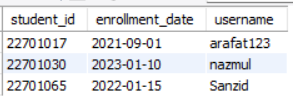
\includegraphics{images/table_data/student_table (1).png}
\end{figure}
\begin{itemize}
    \item \textbf{Functional Dependencies:}
    \begin{itemize}
        \item \texttt{student\_id} $\rightarrow$ \texttt{enrollment\_date, username}
    \end{itemize}

    \item \textbf{Candidate Keys:} \texttt{student\_id}

    \item \textbf{Prime Attributes:} \texttt{student\_id}

    \item \textbf{Non-Prime Attributes:} \texttt{enrollment\_date, username}

    \item \textbf{Analysis:} In this table, all functional dependencies have a candidate key on the left-hand side, fulfilling the conditions of 3NF. There are no transitive dependencies, and all non-prime attributes are fully functionally dependent on \texttt{student\_id}.

    \item \textbf{Conclusion:} The \texttt{student} table is in 3NF.
\end{itemize}

\subsection{Normalizing teacher Table}

The \texttt{teacher} table has the attributes:
\[
\{ \texttt{teacher\_id}, \texttt{employment\_date}, \texttt{username} \}
\]
\begin{figure}
    [h]
    \centering
    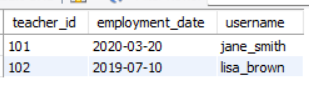
\includegraphics{images/table_data/teacher_table.png}
\end{figure}
\begin{itemize}
    \item \textbf{Functional Dependencies:}
    \begin{itemize}
        \item \texttt{teacher\_id} $\rightarrow$ \texttt{employment\_date, username}
    \end{itemize}

    \item \textbf{Candidate Keys:} \texttt{teacher\_id}

    \item \textbf{Prime Attributes:} \texttt{teacher\_id}

    \item \textbf{Non-Prime Attributes:} \texttt{employment\_date, username}

    \item \textbf{Analysis:} This table meets the conditions of 3NF as all functional dependencies have a candidate key on the left-hand side. There are no transitive dependencies, and all non-prime attributes are fully functionally dependent on \texttt{teacher\_id}.

    \item \textbf{Conclusion:} The \texttt{teacher} table is in 3NF.
\end{itemize}

\subsection{Normalizing venue Table}

The \texttt{venue} table has the attributes:
\[
\{ \texttt{venue\_id}, \texttt{venue\_name} , \texttt{location\_id}\}
\]
\begin{figure}
    [h]
    \centering
    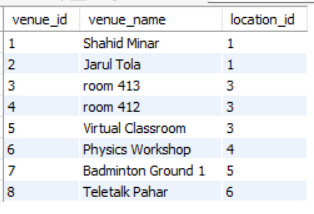
\includegraphics{images/table_data/venue_table.png}
\end{figure}
\begin{itemize}
    \item \textbf{Functional Dependencies:}
    \begin{itemize}
        \item \texttt{venue\_id} $\rightarrow$ \texttt{venue\_name, location\_id}
    \end{itemize}

    \item \textbf{Candidate Keys:} \texttt{venue\_id}

    \item \textbf{Prime Attributes:} \texttt{venue\_id}

    \item \textbf{Non-Prime Attributes:} \texttt{venue\_name,location\_id}

    \item \textbf{Analysis:} The functional dependency has a candidate key 
    (\texttt{venue\_id}) on the left-hand side. This satisfies the conditions of 3NF, 
    and there are no transitive dependencies. All non-prime attributes 
    (\texttt{venue\_name,location\_id}) are fully functionally dependent on \texttt{venue\_id}.

    \item \textbf{Conclusion:} The \texttt{venue} table is in 3NF.
\end{itemize}



\subsection{Normalizing location Table}

The \texttt{location} table has the attributes:
\[
\{ \texttt{location\_id}, \texttt{location\_name} \}
\]
\begin{figure}
    [h]
    \centering
    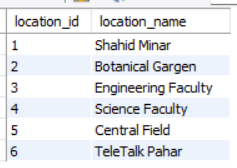
\includegraphics{images/table_data/location_table.png}
\end{figure}
\begin{itemize}
    \item \textbf{Functional Dependencies:}
    \begin{itemize}
        \item \texttt{location\_id} $\rightarrow$ \texttt{location\_name}
    \end{itemize}

    \item \textbf{Candidate Keys:} \texttt{location\_id}

    \item \textbf{Prime Attributes:} \texttt{location\_id}

    \item \textbf{Non-Prime Attributes:} \texttt{location\_name}

    \item \textbf{Analysis:} The functional dependency has a candidate key 
    (\texttt{location\_id}) on the left-hand side. This satisfies the conditions of 3NF, 
    and there are no transitive dependencies. All non-prime attributes 
    (\texttt{location\_name}) are fully functionally dependent on \texttt{location\_id}.

    \item \textbf{Conclusion:} The \texttt{location} table is in 3NF.
\end{itemize}

\subsection{Normalizing event\_category Table}

The \texttt{event\_category} table has the attributes:
\[
\{ \texttt{category\_id}, \texttt{category\_name} \}
\]
\begin{figure}
    [h]
    \centering
    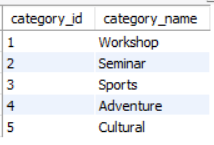
\includegraphics{images/table_data/event_category.png}
\end{figure}
\begin{itemize}
    \item \textbf{Functional Dependencies:}
    \begin{itemize}
        \item \texttt{category\_id} $\rightarrow$ \texttt{category\_name}
    \end{itemize}

    \item \textbf{Candidate Keys:} \texttt{category\_id}

    \item \textbf{Prime Attributes:} \texttt{category\_id}

    \item \textbf{Non-Prime Attributes:} \texttt{category\_name}

    \item \textbf{Analysis:} The functional dependency has a candidate key (\texttt{category\_id}) on the left-hand side, meeting 3NF requirements. There are no transitive dependencies, and all non-prime attributes are fully functionally dependent on \texttt{category\_id}.

    \item \textbf{Conclusion:} The \texttt{event\_category} table is in 3NF.
\end{itemize}

\subsection{Normalizing event Table}

The \texttt{event} table has the attributes:
\[
\{ \texttt{event\_id}, \texttt{event\_name}, \texttt{description}, \texttt{event\_date}, \texttt{start\_time}, \texttt{end\_time}, \texttt{status}, \texttt{max\_attendees}, \texttt{category\_id}, \texttt{venue\_id} \}
\]

\begin{figure}
    [h]
    \centering
    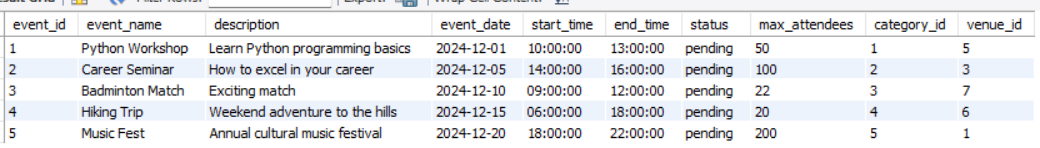
\includegraphics{images/table_data/event.png}
\end{figure}

\begin{itemize}
    \item \textbf{Functional Dependencies:}
    \begin{itemize}
        \item \texttt{event\_id} $\rightarrow$ \texttt{event\_name, description, event\_date, start\_time, end\_time, status, max\_attendees, category\_id, venue\_id}
    \end{itemize}

    \item \textbf{Candidate Keys:} \texttt{event\_id}

    \item \textbf{Prime Attributes:} \texttt{event\_id}

    \item \textbf{Non-Prime Attributes:} \texttt{event\_name, description, event\_date, start\_time, end\_time, status, max\_attendees, category\_id, venue\_id}

    \item \textbf{Analysis:} All functional dependencies have a candidate key (\texttt{event\_id}) on the left-hand side. There are no transitive dependencies, and all non-prime attributes are fully functionally dependent on \texttt{event\_id}, fulfilling 3NF.

    \item \textbf{Conclusion:} The \texttt{event} table is in 3NF.
\end{itemize}

\subsection{Normalizing registers Table}

The \texttt{registers} table has the attributes:
\[
\{ \texttt{username}, \texttt{event\_id}, \texttt{registration\_date} \}
\]

\begin{itemize}
    \item \textbf{Functional Dependencies:}
    \begin{itemize}
        \item \texttt{(username, event\_id)} $\rightarrow$ \texttt{registration\_date}
    \end{itemize}

    \item \textbf{Candidate Keys:} \texttt{(username, event\_id)}

    \item \textbf{Prime Attributes:} \texttt{username, event\_id}

    \item \textbf{Non-Prime Attributes:} \texttt{registration\_date}

    \item \textbf{Analysis:} The only functional dependency has a composite candidate key (\texttt{username, event\_id}) on the left-hand side, fulfilling 3NF. There are no transitive dependencies, and the non-prime attribute \texttt{registration\_date} is fully functionally dependent on the composite key.

    \item \textbf{Conclusion:} The \texttt{registers} table is in 3NF.
\end{itemize}

\subsection{Normalizing organized\_by Table}

The \texttt{organized\_by} table has the attributes:
\[
\{ \texttt{username}, \texttt{event\_id} \}
\]

\begin{itemize}
    \item \textbf{Functional Dependencies:}
    \begin{itemize}
        \item \texttt{(username, event\_id)} $\rightarrow$ \texttt{[no additional attributes]}
    \end{itemize}

    \item \textbf{Candidate Keys:} \texttt{(username, event\_id)}

    \item \textbf{Prime Attributes:} \texttt{username, event\_id}

    \item \textbf{Non-Prime Attributes:} None

    \item \textbf{Analysis:} The table consists only of the composite candidate key (\texttt{username, event\_id}), so there are no additional attributes to check for dependency. Thus, it satisfies 3NF.

    \item \textbf{Conclusion:} The \texttt{organized\_by} table is in 3NF.
\end{itemize}


%\section{System Architecture}\label{sec:sa}
Describe the architecture of your system using a figure: Describe how each component of the architecture communicate. 
\clearpage
%\section{Implementation}\label{sec:imp}
Give some code snippet of each component you outlined in your System architecture. Some DDL query example. Use the listing environment for writing code. 
Listing~\ref{list:sql} shows an SQL query. 

\begin{lstlisting}[caption={A SQL query example}, label=list:sql, captionpos=b,
           backgroundcolor=\color{white},
           language=SQL,
           breaklines=true,
           frame=single,
           showspaces=false,
           basicstyle=\ttfamily,
           numbers=left,
           numberstyle=\tiny,
           rulecolor=\color{red},
           keywordstyle=\color{blue},
           commentstyle=\color{gray}
        ]
select distinct name
from instructor
where salary > some( select salary
			from instructor
			where dept_name='CSE');
\end{lstlisting}
\clearpage

%\section{Validation} \label{sec:val}
Show that users are satisfied with your product. 
You can also give a user manual here describing how to use your system (process of completion of different tasks using your system )
You can use some matrices (time, cost, resource etc.) to compare your system with the previous system. 
\clearpage
%\section{Software Deployment}\label{sec:sd}
Describe how to install and configure your system so that a non-technical user can use your system. 

\clearpage
%\section{Conclusion and Future Work}\label{sec:cfw}
Write the conclusion of your project: what was the problem? what the developed solution offers, Significance of the project, limitations of the project and future work. 
\clearpage











%
%\section{Bibliography} 
%\label{sec:bibliography}
%To add bibliography in your document, use the following steps:
\begin{enumerate}
\item First create a .bib file in the same directory where your .tex file is (in our case, the file name is references.bib). Also place the bibliography style file in the same directory. In our case, we are using the ios1.bst style file. We include the following commands in the .tex file for the style file and bib file: \\
 \texttt{\textbackslash bibliographystyle\{ios1\}} \\
\texttt{\textbackslash bibliography\{references\}} 
\item Import the BibTeX of your book or paper from Google Scholar or other sources into your .bib file. An example of BibTex is shown in Listings~\ref{list:bibtex}.  

\begin{lstlisting}[caption={A BibTeX example}, label=list:bibtex, captionpos=b,
           backgroundcolor=\color{white},
           language=SQL,
           breaklines=true,
           frame=single,
           showspaces=false,
           basicstyle=\ttfamily,
           numbers=left,
           numberstyle=\tiny,
           rulecolor=\color{red},
           commentstyle=\color{gray}
        ]
@article{kopka1995guide,
  title={A Guide to $\{$$\backslash$LaTeX$\}$--Document},
  author={Kopka, H and Daly, PW},
  year={1995},
  publisher={Citeseer}
}
\end{lstlisting}

\item Then, use the name of the BibTex (in Listing~\ref{list:bibtex}, the name is kopka1995guide) in the text of your .tex document where you want to refer it.

\item After saving your .tex document, execute the PDFLaTeX option one time; then execute the BibTeX option; then again execute the PDFLaTeX option for twice; finally, execute the QuickBuild option. Now your document refer the corresponding book or paper. 
\end{enumerate}

\bibliographystyle{ios1}

%\bibliographystyle{plain}
%\bibliography{references}


\end{document}